\documentclass[12pt]{beamer}
\usepackage{utopia}
\usepackage{biblatex}
\bibliography{foo}
\usetheme{CambridgeUS} 
\usecolortheme{beaver}
\usepackage[utf8]{inputenc}
\usepackage{lmodern}
\graphicspath{{picture/}}
 
%Information to be included in the title page:
\title[DynaMIT-Database Infrastructure]
{Historical Database for DynaMIT2.0}

\author{Meng Yue}

\institute[Dep.Automation,Tsinghua]
{Department of Automation,Tsinghua University, China}

\date[August 6, 2016]
{SMART FM-IRG, August 6, 2016}
 
\logo{
\includegraphics[height=1.5cm]{combine-logo.png}}

\AtBeginSection[]
{
	\setbeamertemplate{section in toc}{{\color{red!70!black}\inserttocsectionnumber.}~\inserttocsection}
	\begin{frame}
		\frametitle{Outline}
		\tableofcontents[currentsection]
	\end{frame}
}

\setbeamertemplate{itemize items}{\color{red!70!black}$\blacktriangleright$}

\begin{document} 

\frame{\titlepage}

\begin{frame}
\setbeamertemplate{section in toc}{{\color{red!70!black}\inserttocsectionnumber.}~\inserttocsection}
\frametitle{Outline}
\tableofcontents
\end{frame}



\section{Background}

\begin{frame}
\frametitle{Starting point}
\setbeamerfont{footnote}{size=\tiny}
The aim of the on–line calibration is to use the off–line calibrated parameter
values as starting points and perform a local optimization step towards the unobserved true values\footnote{ Constantinos,A(2004) On–line Calibration for Dynamic Traffic Assignment}.\\ 
\vspace{0.5in}
Precise historical OD flow $=>$ Accurate estimated OD-flow \\

\end{frame}

\begin{frame}
\frametitle{OD-Flow Analysis}
Altered by many factors:
\begin{itemize}
\item rush hour
\item weather
\item holiday
\item ...
\end{itemize}
%TODO Maybe needs a comparison of od flow between morning an noon.
\vspace{0.5in}
Needs to be stratified under several tags
\end{frame}

\begin{frame}
\frametitle{Insights}
\setbeamerfont{footnote}{size=\tiny}
\begin{itemize}
\item Set up database for storage
\item Update historical data with estimated data
\item Provide best-fit historical flow
\end{itemize}
\end{frame}

\begin{frame}
\frametitle{Goal}
To design a program that can automatically \textbf{save} results from the DynaMIT simulation ,\textbf{update} the historical OD-flow and \textbf{render} proper demand input for the real-time DynaMIT simulation.
\end{frame}
%TODO Here needs discussion with HaiZheng.


\section{Implement}
\begin{frame}
\frametitle{Functions}
\begin{itemize}
\item Save DynaMIT input and output files to database
\item Update the exist records in database
\item Render best-fit historical data given by the input parameters of real-time DynaMIT simulation
\item Auto-check and backup
\end{itemize}
\end{frame}


\begin{frame}
\frametitle{Table definition}
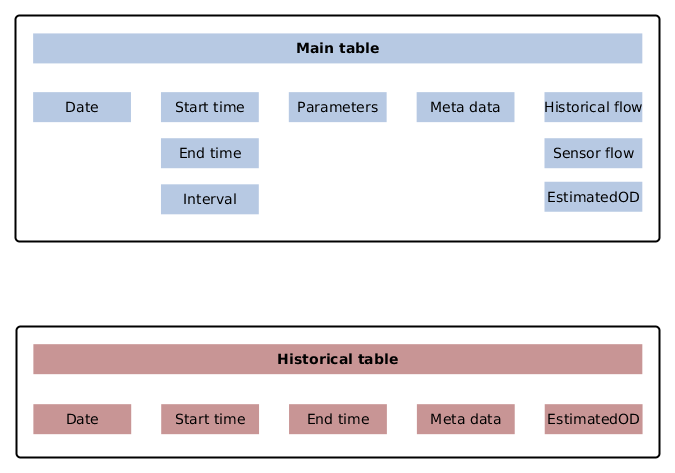
\includegraphics[width = 0.8\textwidth]{table.png}
\end{frame}

\begin{frame}
\frametitle{Flow Diagram}
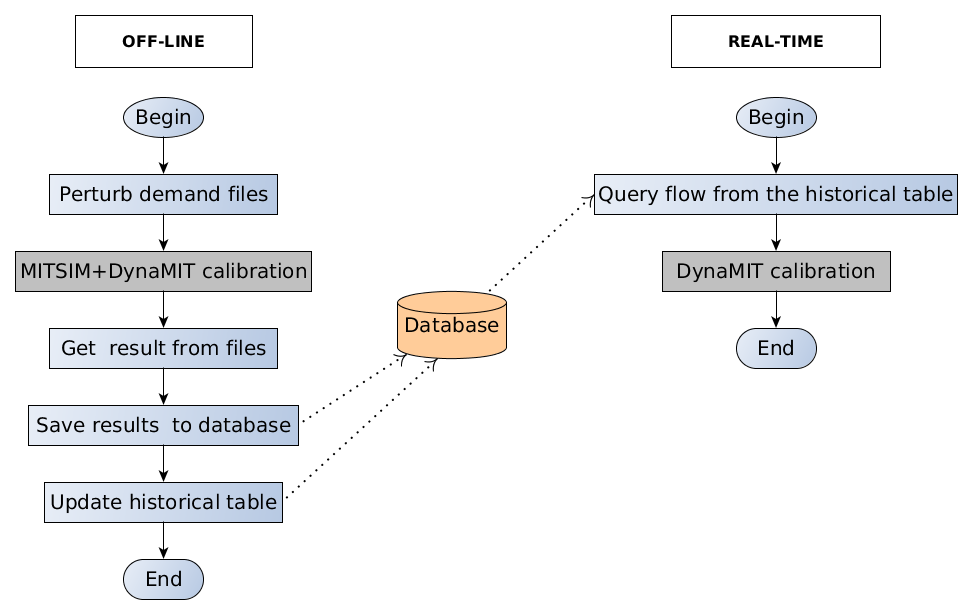
\includegraphics[width = 1.0\textwidth]{flow-chart.png}
\end{frame}

\begin{frame}
\frametitle{Project description}
\begin{itemize}
\item Database: PostgreSQL
\item Language: 
\begin{itemize}
      \item{Python (file operation)}
      \item{Java (database I/D/U/Q)}
      \item{Shell (whole process)}
\end{itemize}
\end{itemize}
\end{frame}



\begin{frame}
\frametitle{Setup process}
\begin{itemize}
\item CREATE TABLE: database.config
\item Framework parameter: params.config \& init.sh
\item Generate demands: demand\_perturb.py 
\end{itemize}
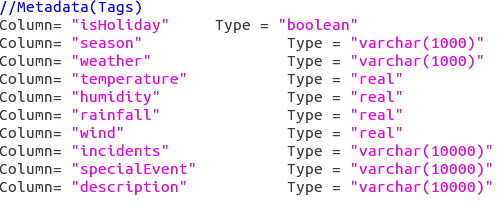
\includegraphics[width = 0.5\textwidth]{screenshot_table.png}
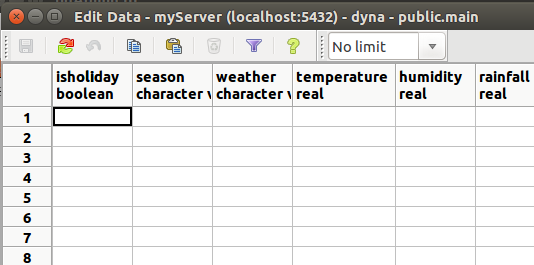
\includegraphics[width = 0.5\textwidth]{screenshot_pgadmin.png}
\end{frame}



\begin{frame}
\frametitle{Insert process(main table)}
\begin{itemize}
\item dtaparam.dat
\item behavior.dat
\item supplyparam.dat
\item sensor.out
\item demand.dat
\item estimatedOD*
\item EOD.txt
\item sen\_flw\_*
\item sen\_spd\_*
\item ...
\end{itemize}
\end{frame}

\begin{frame}
\frametitle{Update process(hod table)}
main::estimatedOD $=>$ hod::historicalOD
\begin{itemize}
\item Last EstimatedOD
\item Moving Average(SMA,EMA)
\item Smoothing Model
\end{itemize}
\end{frame}

\begin{frame}
\frametitle{Generate historical data process}
SELECT estimatedOD FROM hod WHERE ...  
\end{frame}

\begin{frame}
\frametitle{Screen-shot(Start)}
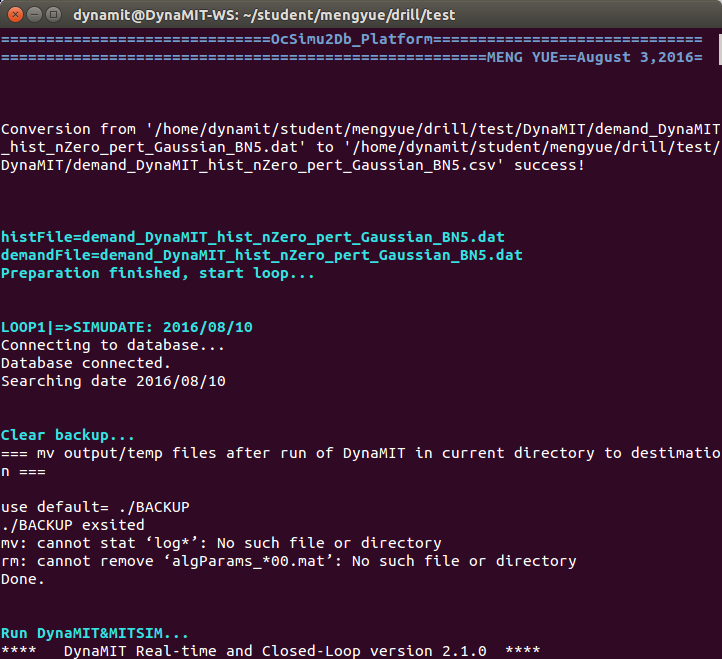
\includegraphics[width = 0.6\textwidth]{screenshot_2.png}
\end{frame}

\begin{frame}
\frametitle{Screen-shot(End)}
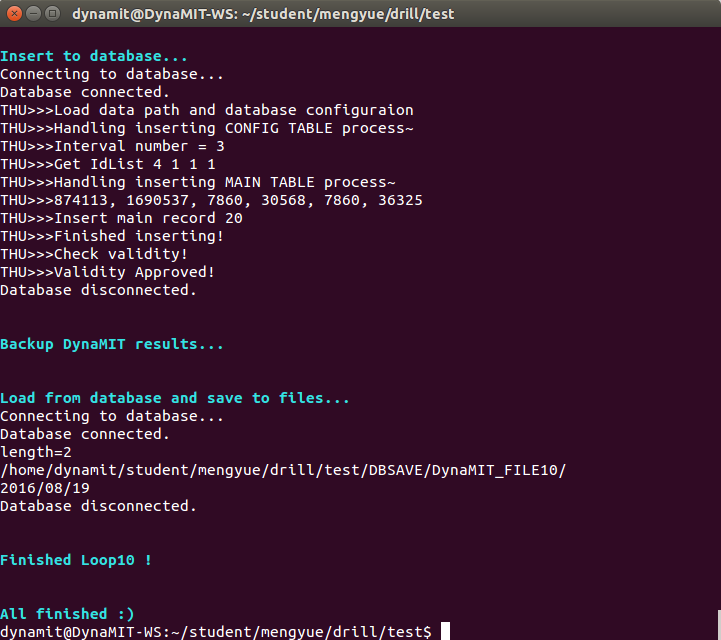
\includegraphics[width = 0.6\textwidth]{screenshot_1.png}
\end{frame}

\begin{frame}
\frametitle{Screen-shot(Error)}
Check for conflict primary key DATE
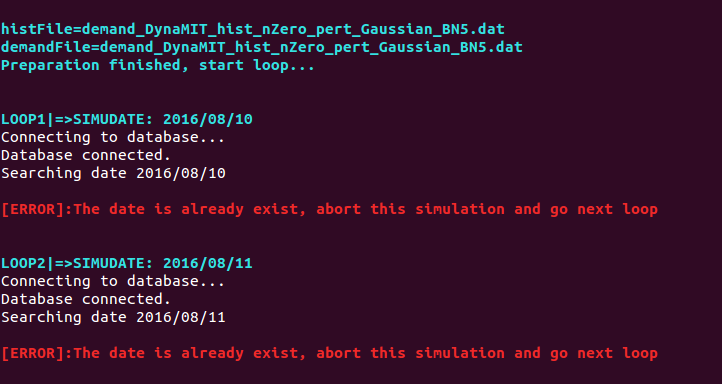
\includegraphics[width = 0.6\textwidth]{screenshot_e.png}
\end{frame}

\section{Test Result}
\begin{frame}
\frametitle{Test}
\begin{itemize}
\item 17:00-17:20,10 DAYS,1633 OD-pairs
\item using different update algorithm()
\item examined by difference output by MITSIM
\end{itemize}
%TODO here we needs a formula.
\end{frame}

\begin{frame}
\frametitle{Result}
\end{frame}

\section{Summary}
\begin{frame}
\frametitle{Conclusion}
\begin{itemize}
\item Run simulation and recording automatically
\item Easy to debug and add new tags for database
\item Potential value
\end{itemize}
\end{frame}

\section{Future work}
\begin{frame}
\frametitle{Future work}
\begin{itemize}
\item Find source for the metadata
\item Use XXX algorithm for "update process"
\item Use XXX algorithm for "render historical data"
\item Refactoring \& Documentation
\end{itemize}
\end{frame}
 
\begin{frame}
\frametitle{Question}
Any questions?
\end{frame}
 
 
\begin{frame}
\frametitle{Thank you!}
\end{frame}
\end{document}

